\chapter{Simulaci\'on de la emisi\'on de radio de las EAS}

\section{ZHAireS}

\section{Caracterizaci\'on de eventos ES}
	
	\subsection{Caracter\'isticas generales}
	
	
	\begin{figure}[ht!]
		\centering
		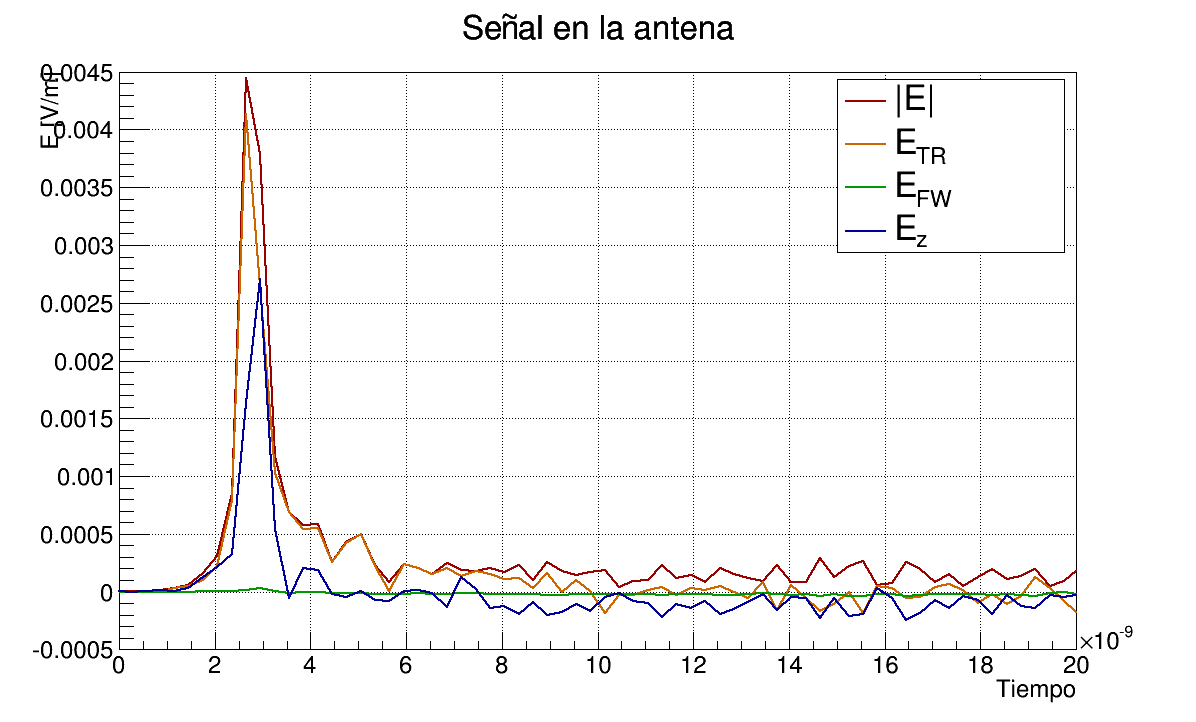
\includegraphics[width=0.8\textwidth]{./fig/simulacionRadio/antennaSignal.png}
		\caption{\label{fig:antSig}
		asd
		}
	\end{figure}
	
	En la figura \ref{fig:testFootprint_E0} se muestra la se\~nal de radio en el suelo para una lluvia simulada en Malarg\"ue, cuyos par\'ametros de simulaci\'on se resumen en la tabla \ref{tab:paramTestShower}
	
	\begin{table}[ht!]
	 \begin{center}
	  \begin{tabular}{ccccc}
	   Canal de decaimiento & $E_v$ & $\theta$ & \xd{} & $\phi$ \\
	   \hline
	   $\tau\rightarrow e^- \nu_{e^-}\nu\tau$ & \cant{10^{18}}{eV} & \cant{90.5}{^\circ} & \cant{25}{m} & \cant{90}{^\circ}
	  \end{tabular}
	  \caption{\label{tab:paramTestShower}
	  as
	  }
	 \end{center}
	\end{table}

	
	\begin{figure}[ht!]
		\centering
		\includegraphics[width=\textwidth]{./fig/simulacionRadio/{foorPrint_ZWv1.22_ntuples_v1.21_ChTest_phi_90_18_89.5_90_25_1238_E0}.png}
		\caption{\label{fig:testFootprint_E0}
		asd
		}
	\end{figure}
	
	\begin{figure}[ht!]
		\centering
		\includegraphics[width=\textwidth]{./fig/simulacionRadio/{foorPrint_ZWv1.22_ntuples_v1.21_ChTest_phi_90_18_89.5_90_25_1238_E0x}.png}
		\caption{\label{fig:testFootprint_E0tr}
		asd
		}
	\end{figure}
	
	\begin{figure}[ht!]
		\centering
		\includegraphics[width=\textwidth]{./fig/simulacionRadio/{foorPrint_ZWv1.22_ntuples_v1.21_ChTest_phi_90_18_89.5_90_25_1238_E0y}.png}
		\caption{\label{fig:testFootprint_E0fw}
		asd
		}
	\end{figure}
	
	\begin{figure}[ht!]
		\centering
		\includegraphics[width=\textwidth]{./fig/simulacionRadio/{foorPrint_ZWv1.22_ntuples_v1.21_ChTest_phi_90_18_89.5_90_25_1238_E0z}.png}
		\caption{\label{fig:testFootprint_E0z}
		asd
		}
	\end{figure}
	
	\subsubsection{Emisi\'on coherente - Cono \cher}
	
	\begin{figure}[ht!]
		\centering
		\includegraphics[width=\textwidth]{./fig/simulacionRadio/{foorPrint_Cone_ZWv1.22_ntuples_v1.21_ChTest_phi_90_18_89.5_90_25_1238_E0}.png}
		\caption{\label{fig:testFootprint_Cone}
		asd
		}
	\end{figure}
	
	\clearpage
	\subsection{Tratamiento de la se\~nal}
	
	\begin{figure}[ht!]
		\centering
		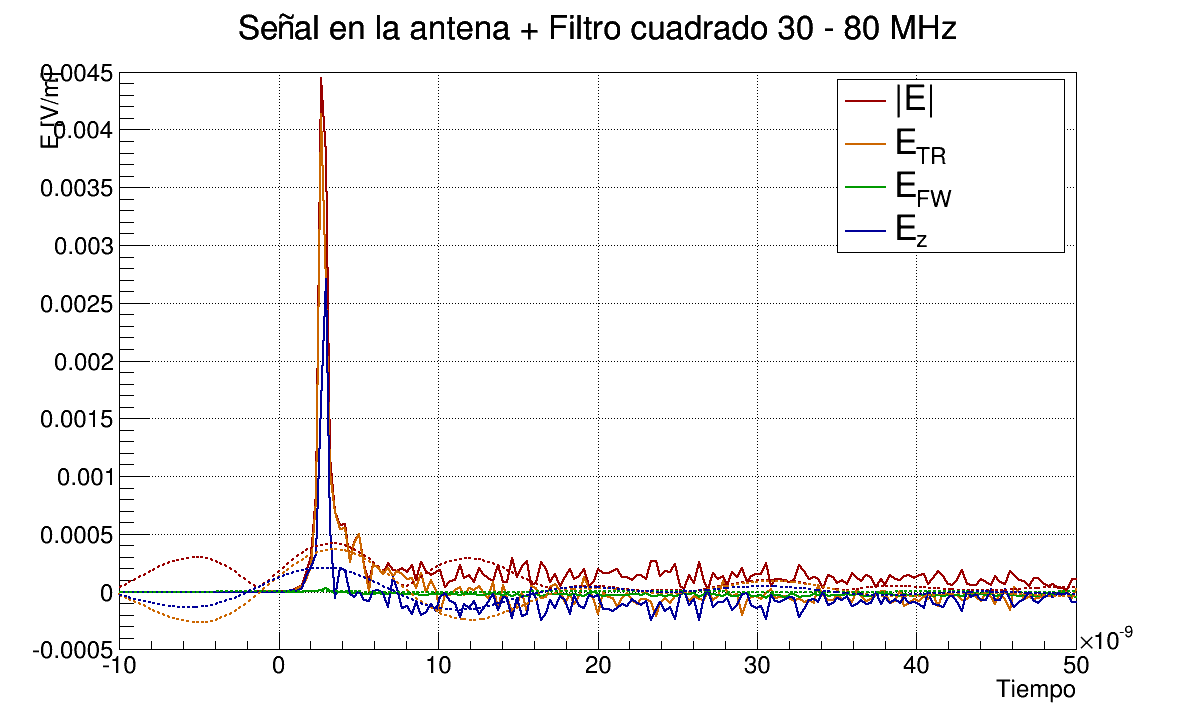
\includegraphics[width=0.8\textwidth]{./fig/simulacionRadio/antennaFilt.png}
		\caption{\label{fig:antFilt}
		asd
		}
	\end{figure}
	
	\begin{figure}[ht!]
		\centering
		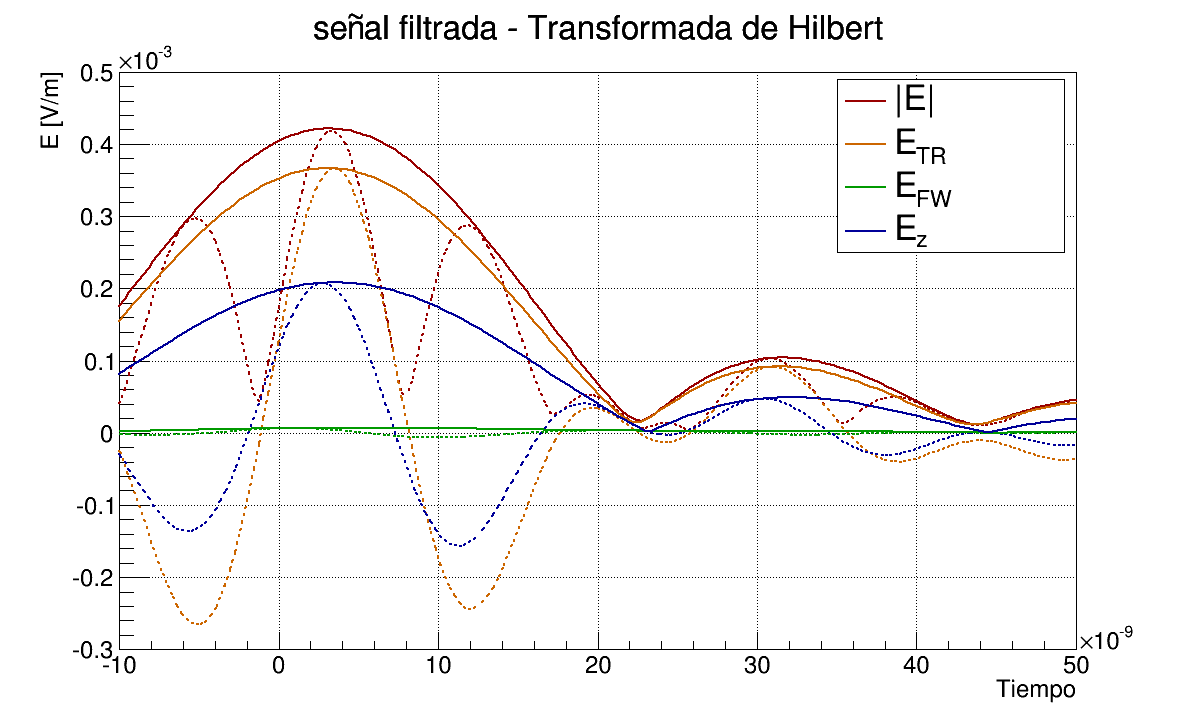
\includegraphics[width=0.8\textwidth]{./fig/simulacionRadio/antennaHEnv.png}
		\caption{\label{fig:antHEnv}
		asd
		}
	\end{figure}
	
	
	\begin{figure}[ht!]
		\centering
		\includegraphics[width=\textwidth]{./fig/simulacionRadio/{foorPrint_ZWv1.22_ntuples_v1.21_ChTest_phi_90_18_89.5_90_25_1238_E}.png}
		\caption{\label{fig:testFootprint_E}
		asd
		}
	\end{figure}
	
	\begin{figure}[ht!]
		\centering
		\includegraphics[width=\textwidth]{./fig/simulacionRadio/{foorPrint_ZWv1.22_ntuples_v1.21_ChTest_phi_90_18_89.5_90_25_1238_Ex}.png}
		\caption{\label{fig:testFootprint_Etr}
		asd
		}
	\end{figure}
	
	\begin{figure}[ht!]
		\centering
		\includegraphics[width=\textwidth]{./fig/simulacionRadio/{foorPrint_ZWv1.22_ntuples_v1.21_ChTest_phi_90_18_89.5_90_25_1238_Ey}.png}
		\caption{\label{fig:testFootprint_Efw}
		asd
		}
	\end{figure}
	
	\begin{figure}[ht!]
		\centering
		\includegraphics[width=\textwidth]{./fig/simulacionRadio/{foorPrint_ZWv1.22_ntuples_v1.21_ChTest_phi_90_18_89.5_90_25_1238_Ez}.png}
		\caption{\label{fig:testFootprint_Ez}
		asd
		}
	\end{figure}
	
	\clearpage
	\subsection{Evoluci\'on de la se\~nal a nivel del suelo}
		
	
	mostrar evolucion del EMax a lo largo de la lluvia
	
	mostrar espectro y evolucion
	
	mostrar fit del maximo de la lluvia como funcion de xd y theta y dependencia con la energia
	
		\subsubsection{Evoluci\'on de la polarizaci\'on}
		
		cambio askaryan geomagnetico?
	
	\subsection{Corte en $\theta$}
	
	plots dado xd para diferentes thetas
	mostrar tomataso
	
	\clearpage
	\subsection{Influencia del campo magn\'etico terrestre}
	
	\begin{figure}[ht!]
		\centering
		\includegraphics[width=\textwidth]{./fig/simulacionRadio/{ZHSEvent_18_89.5_0_25_On_1238_E}.png}
		\includegraphics[width=\textwidth]{./fig/simulacionRadio/{ZHSEvent_18_89.5_0_25_Off_1238_E}.png}
		\caption{\label{fig:testFootprint_Ez}
		asd
		}
	\end{figure}
	
	\begin{figure}[ht!]
		\centering
		\includegraphics[width=\textwidth]{./fig/simulacionRadio/{ZHSEvent_18_89.5_0_25_On_1238_Ey}.png}
		\includegraphics[width=\textwidth]{./fig/simulacionRadio/{ZHSEvent_18_89.5_0_25_Off_1238_Ey}.png}
		\caption{\label{fig:testFootprint_Ez}
		asd
		}
	\end{figure}
	
	\begin{figure}[ht!]
		\centering
		\includegraphics[width=\textwidth]{./fig/simulacionRadio/{ZHSEvent_18_89.5_0_25_On_1238_Ez}.png}
		\includegraphics[width=\textwidth]{./fig/simulacionRadio/{ZHSEvent_18_89.5_0_25_Off_1238_Ez}.png}
		\caption{\label{fig:testFootprint_Ez}
		asd
		}
	\end{figure}
	
		\begin{figure}[ht!]
		\centering
		\includegraphics[width=\textwidth]{./fig/simulacionRadio/{ZHSEvent_18_89.5_0_25_On_1238_Ex}.png}
		\includegraphics[width=\textwidth]{./fig/simulacionRadio/{ZHSEvent_18_89.5_0_25_Off_1238_Ex}.png}
		\caption{\label{fig:testFootprint_Ez}
		asd
		}
	\end{figure}
	
	Bon y Boff
	
	mostrar que los efectos son comparables.
	
	velocidad de drift peque\~na por alra densidad en la atmosfera.
	
	\clearpage
	\subsection{Distribuci\'on de part\'iculas vs. se\~nal de radio}
	
	remarcar que el footprint es mucho mas extenso que la distribucion de particulas
	
	\begin{figure}[ht!]
		\centering
		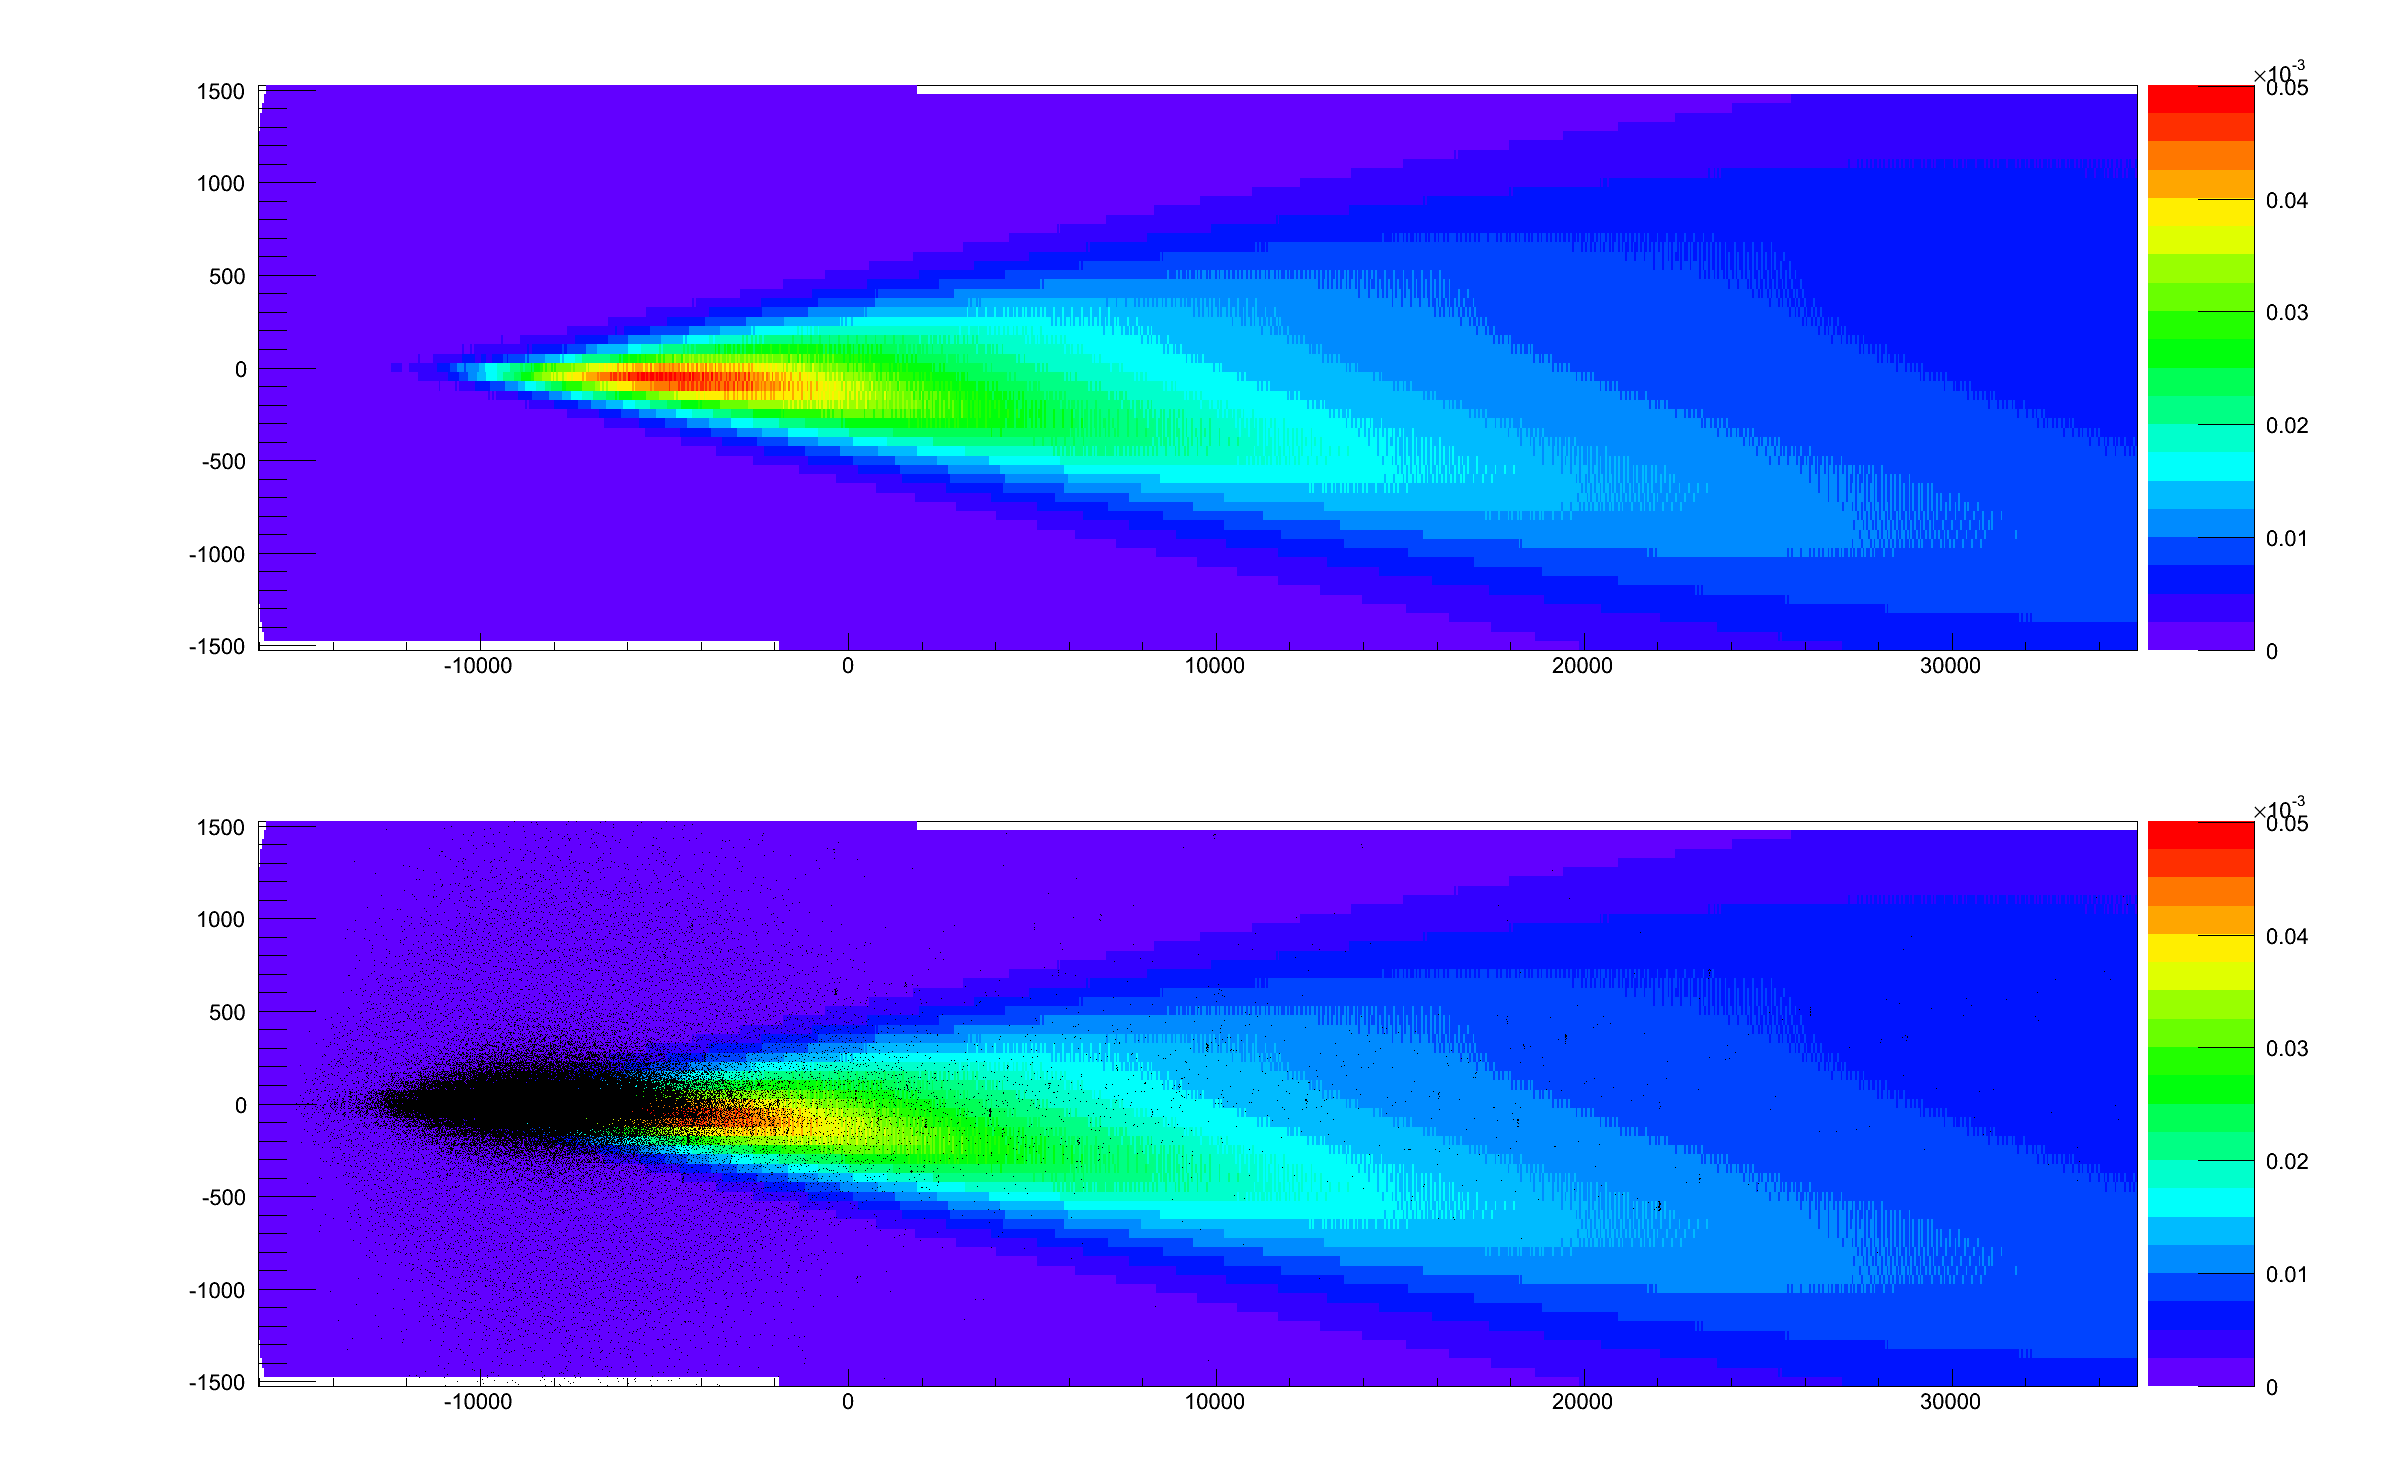
\includegraphics[width=0.8\textwidth]{./fig/simulacionRadio/ZHSEvent_1238_denseArray_E_Particulas}
		\caption{\label{fig:sim_foot_y_part}
		asd
		}
	\end{figure}
	
	\subsection{Dependencia con el canal de decaimiento del \tauon{}}
	
	Graficar distribuciones de diferentes variables que importen para diferentes canales.
	
	Energia visible
	Ancho de la lluvia
	Maximo del footprint
	
	
	

